\documentclass[a4paper]{article}

\title{Sweave Example 1}
\author{Friedrich Leisch}

\usepackage{Sweave}
\begin{document}

\maketitle

In this example we embed parts of the examples from the
\texttt{kruskal.test} help page into a \LaTeX{} document:

\begin{Schunk}
\begin{Sinput}
> data(airquality, package="datasets")
> library("stats")
> kruskal.test(Ozone ~ Month, data = airquality)
\end{Sinput}
\begin{Soutput}
	Kruskal-Wallis rank sum test

data:  Ozone by Month
Kruskal-Wallis chi-squared = 29.267, df = 4, p-value = 6.901e-06
\end{Soutput}
\end{Schunk}
which shows that the location parameter of the Ozone
distribution varies significantly from month to month. Finally, we
include a boxplot of the data, using
%% want an eval=FALSE case and referencing a previous chunk:
\begin{Schunk}
\begin{Sinput}
> boxplot(Ozone ~ Month, data = airquality)
\end{Sinput}
\end{Schunk}

\begin{center}
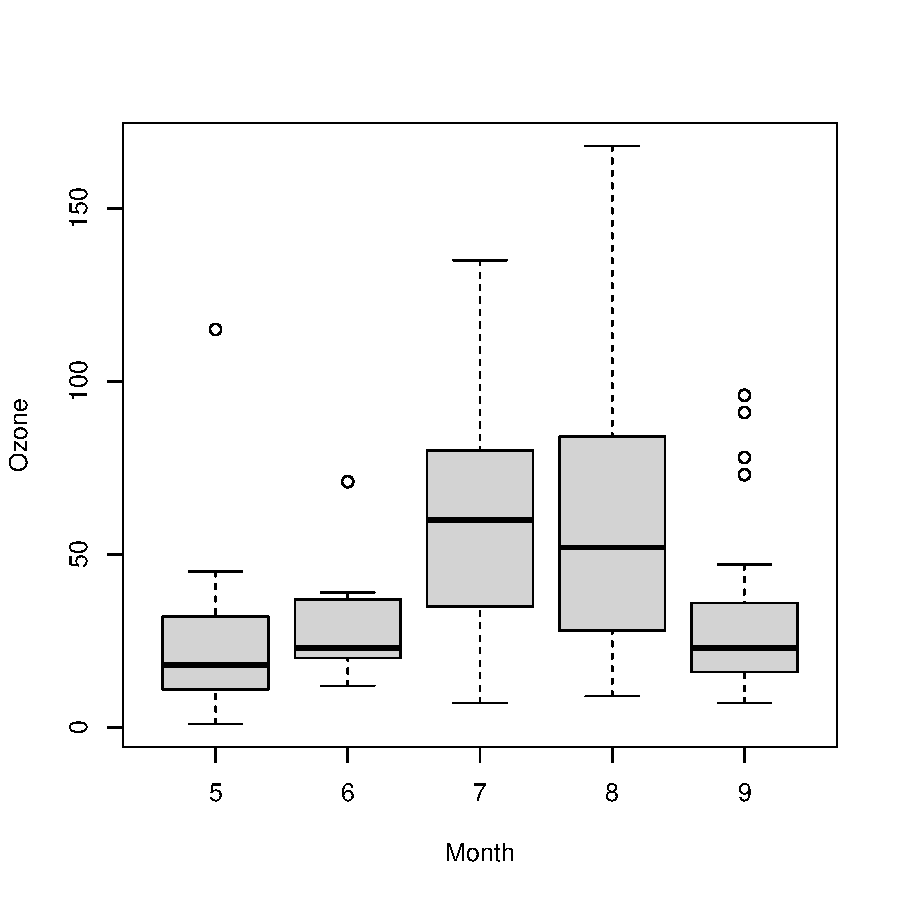
\includegraphics{example-1-003}
\end{center}

\end{document}
